\documentclass[preview]{standalone}

\usepackage{amsmath}
\usepackage{amssymb}
\usepackage{stellar}
\usepackage{definitions}
\usepackage{tikz}
\usepackage{bettelini}

\begin{document}

\id{sequences-functions-convergence}
\genpage

\section{Point convergence}

\begin{snippetdefinition}{function-sequence-convergence-definition}{Convergence}
    Let \(\{f_n\}_{n\in\naturalnumbers}\) be a \sequence of \function[functions].
    The sequence \emph{converges} at a point \(x_0\) if
    \[
        \lim_{n\to\infty} f_n(x_0) \in \realnumbers
    \]
\end{snippetdefinition}

\section{Pointwise convergence}

\begin{snippetdefinition}{pointwise-convergence-definition}{Pointwise convergence}
    Let \(\{f_n\}_{n\in\naturalnumbers}\) be a \sequence of \function[functions].
    The sequence \emph{converges pointwise} to a \function \(f\colon D \to \realnumbers\) if
    \[
        \forall x\in D, \lim_{n\to\infty} f_n(x) = f(x)
    \]
\end{snippetdefinition}

\plain{So the sequence converges at every point, but the speed of convergence may depend on the point.
This definition is very weak.}

\begin{snippetexample}{functions-pointwise-convergence-boundedness-example}{Pointwise convergence and boundedness not preserved}
    Pointwise limits of bounded functions are not necessarily bounded.
    Let \(S = \realnumbers\) be the domain and \(f_n(x) = e^x \chi_{[-n, n]}(x)\), which are bounded.
    The candidate for the pointwise limit is \(f(x) = e^x\), which however is unbounded.
    Let us fix \(x \in S\) and \(\varepsilon > 0\) and look for a natural number
    \(N(\varepsilon, x)\) that satisfies the definition of pointwise convergence.
    We can choose \(N(\varepsilon, x) = \lceil |x| \rceil\), then
    \begin{align*}
        |f_n(x) - f(x)| = 0 < \varepsilon
    \end{align*}
    for \(n > N\).
\end{snippetexample}

\begin{snippetexample}{functions-pointwise-convergence-continuity-example}{Pointwise convergence and continuity not preserved}
    Pointwise limits of continuous functions are not necessarily continuous.
    Let \(S = [-1,1]\) be the domain and
    \[
        f_n(x) = -\chi_{[-1, -\frac{1}{n})}(x) + nx \chi_{[-\frac{1}{n}, \frac{1}{n}]}(x) + \chi_{(\frac{1}{n}, 1]}(x)
        = \begin{cases}
            -1 & x \in \left[-1, -\frac{1}{n}\right) \\
            nx & x \in \left[-\frac{1}{n}, \frac{1}{n}\right] \\
            1 & x \in \left(\frac{1}{n}, 1\right]
        \end{cases}
    \]
    which are continuous.
    \begin{center}
        \begin{tikzpicture}[scale=2]
            \draw[->] (-1.5, 0) -- (1.5, 0) node[right] {$x$};
            \draw[->] (0, -1.5) -- (0, 1.5) node[above] {$y$};

            \draw[dashed, gray] (-1, 0) node[above, text=black] {$-1$} -- (-1, -1);
            \draw[dashed, gray] (1, 0) node[below, text=black] {$1$} -- (1, 1);
            \draw[dashed, gray] (-0.35, 0) node[above, text=black] {$-\frac{1}{n}$} -- (-0.35, -1);
            \draw[dashed, gray] (0.35, 0) node[below, text=black] {$\frac{1}{n}$} -- (0.35, 1);
            
            \draw[dashed, gray] (0, 1) node[left, text=black] {$1$} -- (1, 1);
            \draw[dashed, gray] (0, -1) node[right, text=black] {$-1$} -- (-1, -1);

            \draw[thick, blue] (-1.2, -1) -- (-0.35, -1) -- (0.35, 1) -- (1.2, 1);
            
            \filldraw[blue] (-0.35, -1) circle (0.6pt);
            \filldraw[blue] (0.35, 1) circle (0.6pt);
            
            \node[blue, above] at (0.8, 1) {$f_n(x)$};
        \end{tikzpicture}
    \end{center}
    The candidate limit is \[
        f(x) = -\chi_{[-1, 0)}(x) + \chi_{[0,1]}(x) = \begin{cases}
            -1 & x \in [-1, 0) \\
            0 & x = 0 \\
            1 & x \in (0, 1]
        \end{cases}
    \]
    We also note that this function does not converge uniformly
    because points closer to the origin are more difficult to be approached by \(f_n\)
    relative to points further away.
    Let us fix \(x \in S\) and \(\varepsilon > 0\).
    We want to find \(N(x, \varepsilon)\) that satisfies the definition.
    We can choose an \(N\) such that \(N > \frac{1}{|x|}\).
\end{snippetexample}

\begin{snippetexample}{functions-pointwise-convergence-derivative-example}{Pointwise convergence of the derivatives of a sequence differing from the derivative of the limit}
    Let \(S = \realnumbers\) be the domain and
    \[
        f_n(x) = \frac{\sin(n x)}{\sqrt{n}}
    \]
    Note that \[
        |f_n(x)| \leq \frac{1}{\sqrt{n}} \to 0
    \]
    so \(f_n(x)\) converges pointwise to \(f(x) = 0\).
    However, \[
        f_n'(x) = \frac{n\cos(nx)}{\sqrt{n}} = \sqrt{n} \cos(nx)
    \]
    while \(f'(x) = 0\). The limit of \(f_n'(x)\)
    does not exist for every \(x \in S\) and thus it does not converge pointwise to \(f'(x)\).
\end{snippetexample}

\begin{snippetexample}{functions-pointwise-convergence-integral-example}{Pointwise convergence of the integrals differing from the integral of the limit}
    Let \(S = \realnumbers\) be the domain and
    \[
        f_n(x) = n \chi_{(0, \frac{1}{n})}(x)
    \]
    The candidate limit is \(f(x) = 0\). 
    Let us fix \(x \in S\) and \(\varepsilon > 0\) and we look for a natural number
    \(N(\varepsilon, x)\) that satisfies the definition of
    pointwise convergence.
    We distinguish two cases:
    \begin{itemize}
        \item If \(x \le 0\), then \(x \notin (0, \frac{1}{n})\) for every \(n \ge 1\), thus \(f_n(x) = 0\). We can simply choose \(N = 1\).
        \item If \(x > 0\), in order for the function to vanish we need \(x \ge \frac{1}{n}\), meaning \(n \ge \frac{1}{x}\). We can then choose \(N(\varepsilon, x) = \lceil \frac{1}{x} \rceil\).
    \end{itemize}
    In both cases, for \(n > N\), we get:
    \begin{align*}
        |f_n(x) - f(x)| = 0 < \varepsilon
    \end{align*}
    which proves that \(f_n\) converges pointwise to \(f=0\).
    Both \(f_n\) and \(f\) are Riemann-integrable.
    However,
    \[
        \integral[0][1][f_n(x)][x] = \integral[0][\frac{1}{n}][n][x] = 1
    \]
    while instead
    \[
        \integral[0][1][f(x)][x] = 0
    \]
    which do not coincide. Thus, the numeric sequence
    \[
        \left\{\integral[0][1][f_n(x)][x]\right\}_{n \in \naturalnumbers}
    \]
    does not converge to \(\integral[0][1][f(x)][x]\).
\end{snippetexample}

\plain{We want the sequence of functions to uniformly approximate
its limit function, meaning we want to strengthen the definition
by making the convergence independent of the coordinate.
We want the speed of convergence to be the same at every point.
This allows us to have a convergence that behaves better with respect to boundedness,
continuity, derivatives, and integrals.}

\section{Uniform convergence}

\begin{snippetdefinition}{function-sequence-uniform-convergence-definition}{Uniform convergence}
    Let \(\{f_n\}_{n\in\naturalnumbers}\) be a \sequence of \function[functions].
    The sequence \emph{converges uniformly} to a \function \(f\colon D \to \realnumbers\) if
    \[
        \sup_{x\in D} \left| f_n(x) - f(x) \right| \to 0
    \]
    as \(n\to\infty\).
\end{snippetdefinition}

\plain{Everything that converges uniformly also converges pointwise.}

\begin{snippetexample}{functions-sequence-uniforme-convergence-example}{Uniform convergence of sequence of functions}
    Let \(S = [0, +\infty)\)
    be the domain and \[ f_n(x) = \frac{x}{1 + nx} \]
    The candidate limit is \(f(x) = 0\).
    Let us verify the uniform convergence.
    We have
    \begin{align*}
        \left|f_n(x) - f(x)\right|
        &= \frac{x}{1 + nx} \leq \begin{cases}
            \frac{x}{nx} & x > 0 \\
            0 & x = 0
        \end{cases} \leq \frac{1}{n} \to 0
    \end{align*}
    Therefore it suffices to choose \(N(\varepsilon)\) such that \(N(\varepsilon) > \frac{1}{\varepsilon}\).
    \begin{center}
        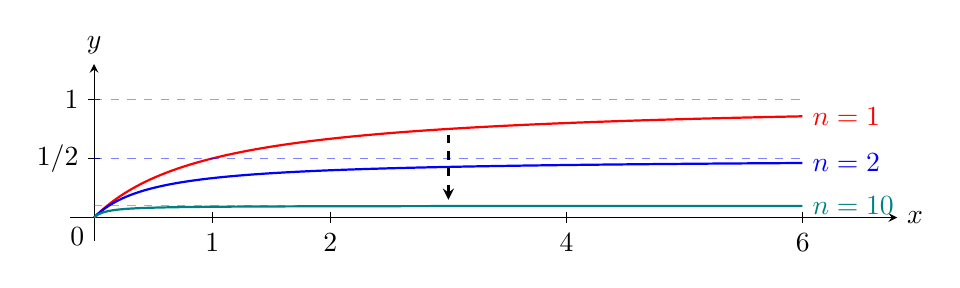
\begin{tikzpicture}[scale=1.5, >=stealth]
            \def\xmax{6}
            \def\ymax{1.3}

            \draw[->] (-0.2, 0) -- (\xmax+0.8, 0) node[right] {$x$};
            \draw[->] (0, -0.2) -- (0, \ymax) node[above] {$y$};

            \draw (1, 0.05) -- (1, -0.05) node[below] {$1$};
            \draw (2, 0.05) -- (2, -0.05) node[below] {$2$};
            \draw (4, 0.05) -- (4, -0.05) node[below] {$4$};
            \draw (6, 0.05) -- (6, -0.05) node[below] {$6$};
            
            \draw (0.05, 1) -- (-0.05, 1) node[left] {$1$};
            \draw (0.05, 0.5) -- (-0.05, 0.5) node[left] {$1/2$};
            \node[below left] at (0,0) {$0$};

            \draw[red, dashed, thin, opacity=0.5] (0, 1) -- (\xmax, 1);
            \draw[red, thick, domain=0:\xmax, samples=200] plot (\x, {\x / (1 + \x)});
            \node[red, right] at (\xmax, {\xmax / (1 + \xmax)}) {$n=1$};

            \draw[blue, dashed, thin, opacity=0.5] (0, 0.5) -- (\xmax, 0.5);
            \draw[blue, thick, domain=0:\xmax, samples=200] plot (\x, {\x / (1 + 2*\x)});
            \node[blue, right] at (\xmax, {\xmax / (1 + 2*\xmax)}) {$n=2$};

            \draw[teal, dashed, thin, opacity=0.5] (0, 0.1) -- (\xmax, 0.1);
            \draw[teal, thick, domain=0:\xmax, samples=200] plot (\x, {\x / (1 + 10*\x)});
            \node[teal, right] at (\xmax, {\xmax / (1 + 10*\xmax)}) {$n=10$};

            \draw[->, black, thick, dashed] (3, 0.7) -- (3, 0.15);
        \end{tikzpicture}
    \end{center}
\end{snippetexample}

\begin{snippet}{sequence-of-function-uniform-convergence-band-condition}
    In general for uniform convergence, we want that \(|f_n(x) - f(x)| < \varepsilon\) \eventually,
    meaning \(f(x) - \varepsilon < f_n(x) < f(x) + \varepsilon\).
    In other words, we want the graphs of \(f_n\) to be \eventually contained
    within the region bounded by the curves \(f-\varepsilon\) and \(f + \varepsilon\).
\end{snippet}

\section{Uniform Cauchy convergence}

\begin{snippetdefinition}{function-sequence-uniform-cauchy-sequence-definition}{Uniform Cauchy sequence}
    Let \(\{f_n\}_{n\in\naturalnumbers}\) be a \sequence of \function[functions].
    The \sequence is \emph{uniformly Cauchy} if
    \[
        \forall \varepsilon > 0,
        \exists N \in \naturalnumbers \suchthat
        \forall n,m > N,
        \sup_{x\in D} \left| f_n(x) - f_m(x) \right| < \varepsilon
    \]
\end{snippetdefinition}

\plain{Starting from a certain index, all functions in the sequence are very close to each other uniformly over the entire domain,
regardless of the limit function.}

\end{document}